\makeatletter
\newif\ifgraphicexist

\catcode`\*=11
\newcommand\IfImageCanBeIncluded[1]{% Taken from https://tex.stackexchange.com/a/99099
    \begingroup
        \global\graphicexisttrue
        \let\input@path\Ginput@path
        \filename@parse{#1}%
        \ifx\filename@ext\relax
            \@for\Gin@temp:=\Gin@extensions\do{%
                \ifx\Gin@ext\relax
                  \Gin@getbase\Gin@temp
                \fi}%
        \else
            \Gin@getbase{\Gin@sepdefault\filename@ext}%
            \ifx\Gin@ext\relax
                \global\graphicexistfalse
                \def\Gin@base{\filename@area\filename@base}%
                \edef\Gin@ext{\Gin@sepdefault\filename@ext}%
            \fi
        \fi
        \ifx\Gin@ext\relax
            \global\graphicexistfalse
        \else 
            \@ifundefined{Gin@rule@\Gin@ext}%
                {\global\graphicexistfalse}%
                {}%
        \fi
        \ifx\Gin@ext\relax 
            \gdef\imageextension{unknown}%
        \else
            \xdef\imageextension{\Gin@ext}%
        \fi 
    \endgroup 
    \ifgraphicexist
        \expandafter \@firstoftwo
    \else
        \expandafter \@secondoftwo
    \fi
}
\catcode`\*=12
\makeatother

% Compile with or without photos
\newif\ifCompileWithPhotos
\CompileWithPhotosfalse

\mode<presentation>
{
    \usetheme{Relax}
    \defbeamertemplate{footline}{Empty}{}
    \setbeamersize{text margin left=8mm,text margin right=8mm}
    %\setbeamerfont{section title}{size=\Huge}
    \defbeamertemplate*{section page}{Iceland}[3][]
    {
        \begin{tikzpicture}[overlay,remember picture, every node/.style={inner sep=0pt}]
            \usebeamercolor{section page background canvas}
            \fill[bg] (current page.south west) rectangle (current page.north east);
            \node[text depth=0.5ex, anchor=west] () (sectionTitle) at ($(current page.north west)+(5mm,-8mm)$)
                  {\usebeamerfont{section title}\usebeamercolor[fg]{section title}\insertsectionhead};
            \node[anchor=north east, inner sep=0] (plan) at ($(current page.north east)-(1mm,1mm)$) {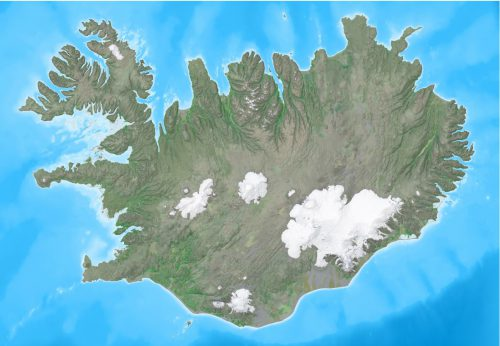
\includegraphics[width=0.21\textwidth, clip, trim=0 0 0 1mm]{Map}};
            \node[anchor=north] (photo) at ($(plan.south west)!0.5!(sectionTitle.south west |- plan.south)-(0,1mm)$) {
                \ifCompileWithPhotos
                    \IfImageCanBeIncluded{#2}{%
                        \includegraphics[width=0.85\textwidth]{#2}
                    }{%
                        \includegraphics[width=0.75\textwidth]{example-image-a}
                    }
                \else
                    \includegraphics[width=0.75\textwidth]{example-image-a}
                \fi
            };
            \node[text depth=0.5ex, below = 2mm of photo.south east, anchor=north east, xshift=-2pt]{#3};
            \ifthenelse{\isempty{#1}}{}%
            {
                \begin{scope}[x={($ (plan.south east) - (plan.south west) $ )},y={( $ (plan.north west) - (plan.south west)$ )}, shift={(plan.south west)}]
                    %\draw[help lines,xstep=.1,ystep=.1] (0,0) grid (1,1);
                    \node[anchor=south, inner sep=0] at (#1) {
\includegraphics[width=2mm]{Pin}};
                \end{scope}
            }
            \ifCompileWithPhotos
                \IfImageCanBeIncluded{#2}{%
                    \node[rotate=90, anchor=west, font=\ssmall] at ($(current page.south east)+(-2mm,1mm)$) {{\raisebox{-2mm}{\Large\textcopyright}} Photo: All rights are reserved};
                }{}
            \fi
        \end{tikzpicture}
    }
    %Add a link to table of content on frames with a footline
    \addtobeamertemplate{footline}{}{%
        \begin{tikzpicture}[remember picture,overlay]
            %xelatex needs \XeTeXLinkBox, won't create a link unless it
            %finds text --- rules don't work without \XeTeXLinkBox.
            %Still builds correctly with pdflatex and lualatex
            \node[anchor=south east, inner sep=2pt] at (current page.south east) {\hyperlink{toc}{\XeTeXLinkBox{
\includegraphics[width=3mm]{TOC}}}};
        \end{tikzpicture}%
    }%
}

\makeatletter
\AtBeginSection[]% <- Empty optional argument, do nothing for \section*
{%
    \ifnum\beamer@tocsectionnumber>0%
        \begin{frame}[plain, noframenumbering]{}
             \sectionpage
        \end{frame}
    \fi
}
\makeatother

%Append code to put third CSC logo on titlepage
\appto\titlepage{%
    \begin{tikzpicture}[remember picture, overlay]
        \node[anchor=south] at (current page.south) {
\includegraphics[width=25mm]{LogoCSC}};
    \end{tikzpicture}
}

%===============================================================%
\title{Introduction to Bash scripting language}
\author{Alessandro Sciarra \\ {\tiny Z02~--~Software Development Center}}
\institute{Organised by the CSC Frankfurt}
\titlegraphic{
\includegraphics[width=20mm]{LogoCRC}}
\titlepagelogo{
\includegraphics[width=20mm]{LogoGoethe}}
%===============================================================%
